\chapter{Case Studies and Applications of e-government system}

\section{Nepal}
\subsection{Cyber Laws}
Cyberlaw is the generic name given to the laws governing the acts that happen and exist in the intangible digital world. The cyberlaws govern aspects such as giving a legal status to the intangible information that exist in the cyberspace, the security and privacy of such information, the relationships and contracts between persons who exchange such information, their rights and responsibilities, crimes relating to damages caused to cyber information and digital assets and all such matters related to the digital world. Cyberlaws are significant and valid not only for regulating cyber matters within countries and states, but are equally essential for resolving issues that arise in cross-national transactions. The need for cyberlaws arises from the singular fact that the laws made for the corporeal world do not take care of several of the actions that happen in the cyberspace.

\subsubsection{Need For Cyberlaw}
\begin{itemize}
	\item Protection of Public Order and Decency
	\item Protection of Privacy of Individuals
	\item Providing Legal Status to Digital Identities and Transactions
\end{itemize}

\subsection{ICT Development Project}

Asian Development Bank(ADB) and the Government of Nepal(GoN) entered a Grant agreement on May $23^{rd}$ 2008 with amount of US \$ $ 2,50,00,000 $ (\textnp{२ करोड ५० लाख डलर}) for the ICT Development project. GoN matched the grant by adding an amount of \$ $ 62,00,000 $ for the project. The outcome of the project was to:

\begin{itemize}
	\item Make ICT more accessible, affordable, inclusive, sustainable, and useful to remote and rural communities.  
	\item Make public services more citizen-centric and business-friendly through ICT.  
	\item Improve accessibility, efficiency, and transparency in Government service delivery with the application of ICT.  
	\item Enhance ICT business and industry.
\end{itemize}

The Project comprised of the following Parts: 

\begin{steps}[label=\textit{PART} \arabic* :]
	\item \textbf{Rural e-Community }
	\begin{itemize}
		\item Wireless Broadband Network
		\item Village Networks
		\item Tele-centers
		\item Community Mobilization and Capacity Development 
	\end{itemize}
	\item \textbf{Government Network}
	\begin{itemize}
		\item Government Information and Data Center
		\item Government Groupware 
	\end{itemize}
\item \textbf{e-Government Applications }
\begin{itemize}
	\item Government Enterprise Architecture
	\item National Identification System
	\item Public Service Recruitment Management System
	\item Land Records Management System
	\item Online Vehicle Registration and Driving Licenses 
\end{itemize}
\item \textbf{Human Resource Development for e-Governance}
\begin{itemize}
	\item Build awareness, knowledge and skill of stakeholders
	\item Establish computer labs for capacity development of 
	training institutions
	\item Revise existing training curriculum of training institutions  etc.
\end{itemize}
\end{steps}

The project has been revised on 28 February, 2013. The Rural e-Community part of the project from the scope of ADB’s ICT Development Project has been excluded from the project plan mainly due to duplication of effort from other Government and private sector.

\subsubsection*{Some G2C Projects of e-Government}

\begin{itemize}
	\item NID Implementation
	\item E-Registration System
	\item Online Passport Application System
	\item Social Insurance Information System
	\item e-Vehicle Registration
	\item e-Driving License  Examination
	\item e-Pension etc
\end{itemize}

\subsubsection*{Some G2B Projects of e-Government}
\begin{itemize}
	\item Central e-Procurement system
	\item e-Customs 
	\item Online Business Registration, renewal and approval management system 
	\item Public service recruitment, training and employment information system
\end{itemize}

\subsubsection*{Some G2G Projects of e-Government}
\begin{itemize}
	\item Formulate directive and perform IT Audit of government IT Systems
	\item Test  existing and upcoming government software to ensure that they meet
	\item e-Tax
	\item Immigration Management System
	\item e-Land
	\item e-MIS, Groupware, e-Pollution, e-Authentication, KMS and GIS
\end{itemize}
\begin{enumerate}
	\item \textbf{National Portal}:
	It is a government website that will act as the single window (one-stop-shop) for all government e-Services and electronic information of Nepal to be delivered to citizens (G2C), business (G2B) and government employees (G2E). Delivery of e-Services will enable increased citizen participation and attempt to create an open, transparent environment through integration of different government information systems and services.
	
	\item \textbf{Inland Revenue Department (e-VAT, e-PAN, e-Filling, e-TDS)}:
	The IRD is responsible for the administration of Value Added Tax, Income Tax, and Excise Duty. All these taxes can now be entered online through the web application developed by IRD. This has made taxpayers job easier.
	
	\item \textbf{Department of Foreign Employment}:
	All the information of Department of Foreign Employment is made public and put in the website. It has an online application to track the record of an foreign employee through their passport number and permit number. 
	
	\item \textbf{Machine Readable Passport}: 
	 Department of Passport has been issuing Machine Readable Passports (MRPs) as per the guidelines of ICAO Machine Readable Travel Document. To effectively carry on this job, the Ministry of Foreign Affairs has awarded the contract to `Oberthur Technologies' of France, a globally renowned company in the field of smart card technology and associated services, which personalizes the Nepalese Machine Readable Passports to the Department of Passport. 
	 
	 \item \textbf{Government Accounting System (FCGO)}: Financial Comptroller General Office (FCGO) is the main agency responsible for the Public Financial Management (PFM) system of Government of Nepal (GoN). IT based Government Accounting System (CGAS) has also been designed and is executed. This captures transactions and their accounting, book keeping, reporting in respect of expenditure, revenue, and retention money in these units. 
	 
	 \item \textbf{e-Procurement}: 
	  PPMO has developed an online portal for all the works related to public procurement. It has a portal \url{https://bolpatra.gov.np} which gives a web interface for all services. E-procurement web portal of is designed to facilitate the bidder to submit their bids through e-submission. 
	  
	  \item \textbf{Public Service Commission}: 
	  Many processes of Public Service Commission are now going online. It includes online application, result viewing etc. 
	  
	  \item \textbf{National ID}:
	  National ID project is aimed at providing a single identification smart card to all the citizens which will contain all information regarding the citizen. 
	  
	  \item \textbf{e-Passport}: e-Passport is aimed at digitizing the current passport system. All the information regarding citizen's passport will be available digitally via online application. 
\end{enumerate}



\subsection{Government Integrated Data Center (GIDC)}
It's a National Data Center for Nepal for the first time in the whole history of ours, built with the help
of the KOICA, Korean Government. The name given for this Data Center is Government Integrated
Data Center (GIDC). This project was started on $ 14^{th} $ May, 2008.


It has mainly three types of Data Centers:
\begin{itemize}
	\item \textbf{Internet Data Center (IDC)}: It provides data and Internet services for other companies 
	\item \textbf{Storage Data Network (SDN)}: It is network of interconnected storage devices and data servers usually located within an
	enterprise data center or as an off-site facility offering leased storage space.
	\item \textbf{Enterprise Data Center (EDC)}: This is the central processing facility for an enterprise's computer network.
\end{itemize}


\subsubsection*{Objectives}
The objectives of GIDC are:
\begin{itemize}
	\item Minimize investment cost by using GIDC based common facilities
	\item Improve stability and efficiency through concentrated central management within Data Center that provide Internet access and management for e-government
	\item Minimize operation cost by means of centralized GIDC
	\item Offer easy expansion and upgrade for increasing demands
	\item Offer basic environment for government co-location and integrated government mailing service
\end{itemize}

\subsubsection*{Features}
Features of GIDC:

\begin{itemize}
	\item High End Computing Infrastructure
	\item Storage Area Network (SAN)
	\item High Speed Local Area Network
\item Multi-Tier Security
	\item High Speed Internet Connectivity
\item $ 24 \times 7\times 365 $ Help Desk
\item Multi level redundant power back-up
\item Air Conditioning Management
\item Fire Detection \& Control System
\end{itemize}

\subsubsection*{Facilities}
Facilities of GIDC:

\begin{enumerate}
	\item \textbf{Information Technology System}:
	\begin{itemize}
		\item Routers, Backbone Switches etc.
		\item Integrated Network Management System
		\item Integrated Server Management System
		\item Integrated Storage
		\item Integrated Back-up
		\item High level firewall with security for different attacks and threats
	\end{itemize}
\item \textbf{Infrastructure System}:
\begin{itemize}
	\item Air-Circulation System : HVAC (Heating, Ventilating, and Air Conditioning)
	\item Security: Biometric Access Control System, Card Reader Access Control System, CCTV
	\item Main Monitoring Room: Integrated Console
	\item Facility Management System: Water Leakage Sensing
	\item Disaster Prevention System: Fire-Fighting
\end{itemize}

\item \textbf{Electrical System}:
\begin{itemize}
	\item Auto Load Transfer Switch
	\item Main Power Switchboard (3 Transformers)
	\item Emergency Generator: $ 400 KW $
	\item UPS: $ 200KVA $
	\item Batteries: $ 480 nos $.
\end{itemize}
\end{enumerate}

\subsubsection*{Security}
To guard against line failure or intrusion, the data center is staffed $ 24 $ hours a day. Movement
throughout the facility is escorted at ALL times. There is $ 24 \times 7 $ closed circuit monitoring of all areas
and entrances. Between the cameras, access control, and the security team, the data center facilities are
pretty secure. Along with the physical security there is multi layered logical security system to prevent
any data loss. There are high level firewall devices to limit access to different services and logging
devices to keep track of everything that is happening inside the system.


% TODO: \usepackage{graphicx} required
\begin{figure}[tph]
	\centering
	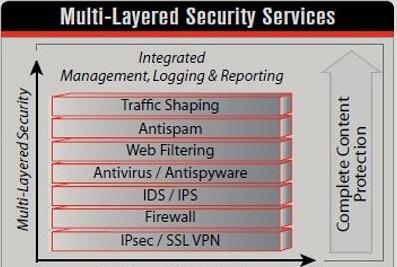
\includegraphics[width=0.8\textwidth]{gidc-sec}
	\caption{GIDC security features}
	\label{fig:gidc-sec}
\end{figure}

The Figure \ref{fig:gidc-sec} shows the different
levels of logical security for the
protection of data inside NITC. There
are seven layers of Security Services
provided by NITC including firewall
and anti-spam security. These layers
provide complete content protection
along with integrated management,
logging \& reporting.

\subsection{e-Government Master Plan}
The e-Governance Master Plan for the Government of Nepal was previously
formulated by Korea IT Industry Promotion Agency (KIPA) working with the then High Level Committee for
Information Technology (HLCIT) for the years 2007 ‐ 2011. KIPA had signed a MOU with the then High Level Commission for Information Technology (HLCIT) for the said task.

\subsubsection*{eGMP2}
After a rigorous review and analysis of the e‐Government Master Plan 2007 -- 2011 and analysis of the prevailing
policies, acts and regulations concerning ICT and e‐Governance, the team determined areas that required
intervention and update and projects that need to be implemented for e ‐ Governance to be successfully realized in
Nepal.

\subsubsection*{Four pillars of eGMP2}
\paragraph*{Sustainability}
\begin{itemize}
	\item Demand Responsive / Self-ownership Projects (Bottom Up Approach)
	\item Shared Benefits (Citizen / Business, Government / Employees, Social / Economic)
	\item Services outsourced / Local Technical Availability
	\item Assurance of AMC 
\end{itemize}

\paragraph*{Capacity building}
\begin{itemize}
	\item Awareness Campaigns (Citizen/Business) 
	\item Chief Information Officers (CIO) in every Government of Nepal (GON) Centers \& IT Cell
	\item HRD and Motivation
\end{itemize}

\paragraph*{Service delivery}
\begin{itemize}
	\item Client satisfaction surveys
	\item Rewards for accomplishes
	\item Use of new technology and media for better deliver
\end{itemize}

\paragraph*{Implementation}
\begin{itemize}
	\item Top Management Commitment
	\item Motivation for efficiency in work
\item Monitoring and Evaluation (M\&E)
\end{itemize}

\subsection{Human Resource Management Software}
\begin{framed}
	\begin{center}
		\begin{nepali}
			यो शीर्षक अस्पष्ट भएकाले कुनै सामग्री फेला पार्न सकिएन।
		\end{nepali}
	\end{center}
\end{framed}

\section{India}

\subsection{Community Information Centers}
A project of connecting the blocks of the District through ICT was launched in 2000 and accordingly a Community Information Centre (CIC) were also setup in Dibang Valley District. Under Phase-1 project, Mipi-Anini-Aliney Block was selected setup. Under various natural stress and strain, the project was completed in 2002 and have been operational since then. The main feature of the CIC has been the internet and email services provided in such mountainous and terrain geography where telephone service is a far off dream for a common man. The rural youths can now get connected to the rest of the world with a click of button and get any information needed. For example, when the CBSE results were declared, the students got their results sitting in their schools or Block Hqr within no time. Prior to setting up of CIC, they had to face the hardship of making long journeys to Roing, in Lower Dibang Valley District and then stand on long queues to know their results, or they had to wait for more than a month for the results to arrive at their school. Another benefit has been confirming train reservation status्\footnote{\url{https://dibangvalley.nic.in/egov-initiatives/cic/}}.


\subsubsection*{Objectives}
The project aims to achieve the following objectives:

\begin{multicols}{2}
	\begin{itemize}
		\item ICT Infrastructure at Block level
		\item Web Access and Internet Services such as E-mail
		\item Market Access and E-commerce
		\item Access to Socio-Economic Databases
		\item E-learning (Computer Aided Learning Processes) and E-education
		\item E-medicine, E-consulting
		\item E-governance applications, Government to Citizen (Citizen Centric) services
		\item Weather Information
		\item IT awareness among local people
		\item Computer Training Programmes
		\item Tender Notification
		\item E-employment Notification
	\end{itemize}
\end{multicols}

\subsubsection*{Infrastructure and Management}
The Centre is well-equipped with infrastructure including one server machine, five client systems, one each of a VSAT, Laser Printer, Dot Matrix Printer, modem, LAN hub, TV, Webcam and two UPS (1KVA, 2 KVA). The CIC is looked after by CIC Operators (CICOs) for managing the centres and providing services to the public.

The project is a joint effort by Department of Information Technology (DIT) under Ministry of Communications and Information Technology (MCIT, now Ministry of Electronics \& Information Technology-MEITY), National Informatics Centre (NIC) and the State Governments of the North-Eastern states.

DIT  funded the project and had the responsibility of overall monitoring and management. NIC was the Implementation agency. Application Software development and Training of CIC Operators were a part of NIC’s responsibilities. The State Governments were entrusted with the mandate of site selection, preparation and maintenance, manpower recruitment and identification and creation of content for various services/applications to be delivered through the CIC.

\subsubsection*{Future Plans}
It is proposed to use the Community Information Centres for e-Entertainment in the future. A select bouquet of channels could be telecast through the VSAT based network as TVs with other associated infrastructure is already available at the CIC. Other future prospects are the provision of connectivity to Schools and Block Offices.

\subsection{e-Procurement in The Government of Andhra Pradesh}
The state of Andhra Pradesh identified e-procurement as a core e-government project with a view to introducing transparency and accountability in its procurement operations which amount to about \(\$ 2\) billion (\textnp{२ अरब डलर}) annually. It is decided to adopt a \gls{ppp} model for implementation of the concept. After evaluating the proposals of the 12 e-procurement players in the world, it selected the affiliate of Commerce One in India — C1 India Ltd.\ — to implement the project.

C1 India, set up the required infrastructure and hosted the e-procurement marketplace. Initially, four major procuring agencies, dealing with public works, medicines, computers and transportation were selected for the pilot. The scope of the pilot includes registration of suppliers, market making, training of the suppliers and employees of the buying agencies and introduction of end-to-end procurement capabilities in the portal. The current features include online notification of all tenders, online filing of tenders, auctions and reverse auctions. The partner gets compensated at a fixed percentage of the value of goods and services procured.

The e-Procurement project of Andhra Pradesh, went on to expand its purview to serve over \(90\%\) of the procurement Government. It evolved into a sophisticated system with enhanced security features, analytical capabilities and a digital signature requirement that is mandatory for all users-buyers and suppliers as well. The project continues to be vibrant and is serving the increasing online procurement needs of the Government.

\subsection{e-Suvidha}
E-Suvidha Project has been envisaged with the main aim of benefiting urban citizens at each district of the state and to offer various governmental services both at city as well as district level within the state. Its main objectives are as follows:

\begin{itemize}
	\item To provide ‘Single window all utilities’ system at all the counters of the systematic and well integrated Citizen Service Centres (E-Suvidha Centre) installed at prime locations within the state adjacent to public houses and workplaces that offers computerized information regarding various government departments, semi-government departments, institutional departments, authorized organizations, self-financing departments, integrated information related to selected corporations and bodies, allows settlement of bills, Government payments (G2C) and  professional services of private entities (B2C) through the use of information technology.

	\item To benefit the urban citizens with the above stated services in all the districts of the state and to offer various governmental services both at city and district level.
\end{itemize}

This project has been established as the subordinate official society of \gls{it} and Electronics Department, Government of Uttar Pradesh under Societies Registration Act 1860, and is popularly known as E-Suvidha.

Under E-Suvidha Project citizens are offered various bill payment services of different departments all at one place i.\ e.\ at e-suvidha centre where ‘Single Window all Utilities’ system is followed whereby citizens don’t have to visit different departments for submitting the bills. Presently, this facility is operated through setting up of intranet but in near future it has been proposed that all the services would be made available to the citizens on their residences only via internet.


\subsubsection*{Vision}
The vision of e-Suvidha project is “to provide to the citizens of Uttar Pradesh, all G2C and G2B   One-Stop services and information of Departments and agencies of Central, State and Local Governments in an efficient, reliable, transparent and integrated manner on a sustained basis, with certainty, through easy access to a chain of computerized Integrated Citizen Service Centers (ICSC’s) and through multiple delivery channels like Electronic Kiosks, mobile phones and the Internet”.
The vision of e-Suvidha is to eventually bring all the G2C, G2B and B2C services within the purview of the project as a single interface to obviate the need for citizens and business people to visit the Government offices except for specialized and complex services

% \subsubsection*{Mission}
% The Mission of e-Suvidha Project is “to be the One-Stop-Shop for all C2G interactions”.

% \

\subsubsection*{e-Suvidha Services}
\paragraph*{G2C Services}

\begin{multicols}{2}
	\begin{itemize}
		\item Revenue Department
		\item Urban Development Department
		\item Medical \& Health Department
		\item Social Welfare Department
		\item Women Welfare \& Child Development Department
		\item Handicap Welfare Department
		\item Employment Department
		\item Food \& Civil Supplies Department
		\item Panchayati Raj Department
		\item Labour Board
		\item All Concerned departments with respect to e-District
	\end{itemize}
\end{multicols}


\paragraph*{B2C Services}
\begin{multicols}{2}
	\begin{itemize}
		\item PAN Card
		\item Aadhar Card
		\item LIC Premium Collection
		\item Mobile Top-up/Recharge
		\item Internet Data Card Recharge
		\item Mobile bills payment
	\end{itemize}
\end{multicols}


\section{Other Countries}
\begin{framed}
	\begin{center}
		\begin{nepali}
			परीक्षा नजिकिएकाले यी शीर्षक भित्रका कुनै पनि सामग्री खाेजतलास गरिएन।
		\end{nepali}
	\end{center}
\end{framed}

\subsection{E-Government Development in South Korea}
Assignment

\subsection{e-Government in China}
Assignment

%Although China is not among the top 50 in the United Nation’s 2012 ranking of national e-
%government performance—it ranks 78th—Chinese leadership has increasingly encouraged e-
%government programs, which have outpaced China’s economic and demographic peers. In
%2012, a UN survey labeled China’s e-government gains “impressive.”
%
%Chinese e-government may also help address the staggering disparity between rural and urban
%Chinese. Many commentators argue that the large gaps between rural and urban income,
%services and infrastructure in China—some of the world’s most drastic—can be addressed by
%closing the “digital divide” between the two regions.
%
%Central government is employing the Internet as an instrument to assist or accelerate the
%process of reformation and to efficiently implement some political measures. The e importance
%of e-government in China is now acknowledged. By introducing a rational and transparent e-
%government, the Chinese government has taken a significant step towards technical legitimacy,
%even if the government’s fate cannot be predicted.
%E-government services are now available in more than 90 percent of China's cities and 80
%percent of its towns, Vice President of the Chinese Academy of Governance Hong Yi said
%Thursday.
%
%All central government departments and provincial-level governments have established
%websites and 99.1 percent of municipal governments have done the same. Over 90 percent of
%core central government services, such as those relating to customs, taxation, public security
%and social security, are now offered online.
%
%Chinese e-government services have seen progress in terms of networking, infrastructure,
%digitalization, sharing and security over the last decade
%Despite several efforts in recent years, weak infrastructure and poor education levels of the
%rural population have continued to hamper the promotion of the Internet in the countryside,
%Therefore, the Chinese Government was now exploring different and more pragmatic methods
%to improve e-governance in these areas, rather than merely trying to spread the use of the
%Internet.


\subsection{e-Government in Brazil}
Assignment

\subsection{e-Government in  Sri Lanka}
Assignment

%The Government Information Centre (GIC) was established as Sri Lanka’s first one-stop
%Government call centre under the Re-engineering Government Programme in August, 2006 to
%enable citizens to obtain Government information and services in an efficient, effective and
%friendly manner. The GIC was launched as a public / private sector partnership and it is
%a single, electronic, trilingual, online knowledgebase of over 1,500 services available from more
%than 120 key Government organizations.
%
%By using GIC (call centre), general public can obtain accurate information immediately. It is
%easy, time saving and the information about many services can be obtained from one place.
%There is no need to visit Government institutes to get information, no need to wait and waste
%time in institutions to obtain information; hence it saves time and expenses during the visits.
%Ultimately the GIC helps people to make their day to day work easier by minimizing the burden
%of obtaining information on Government services.
%
%The Government of Sri Lanka (GoSL) launched “e-Sri Lanka”, a national development initiative in
%November 2002, with the aim of enhancing growth and equity through: (1) improved access
%and use of information and communication technology; (2) access to and use of public services
%on-line by businesses and citizens; and (3) enhanced competitiveness of the private sector and
%in particular of knowledge industry and small and medium enterprises (SMEs).
%
%e-Sri Lanka is a roadmap with the objective of harnessing ICTs towards achieving socio-
%economic development in the country. It is comprised of six core programmes: Re-Engineering
%Government, e-Society, ICT Policy, Leadership and Capacity Building, Information Infrastructure,
%and ICT Investment and Private Sector Development.
%
%Specifically the project work supports (1) establishing an effective, citizen centered and
%business friendly government; (2) empowering the rural poor, disadvantaged groups, women
%and youth through increased and affordable access to information and communication tools
%developing leadership and skills in ICT; and (3) creating employment in the ICT industry and ICT
%enabled services, and enhancing the competitiveness of user industries and services.
%The project comprises the following component Programmes:
%
%- ICT Policy, Leadership and Institutional Development Programme
%- ICT Human Resource Development and Industry Promotion Programme
%- Backbone Communications Infrastructure
%- Tele-Centre Development Programme
%Re-engineering Government Programme
%- e-Society Programme
%
%Government Organizations are the main stakeholders of GIC project. At present over 120
%Government Institutes are linked with GIC and the information on services of those
%organizations are available in GIC knowledgebase. GIC activities in Government Organizations
%are coordinated through a “GIC Coordinator”, who is appointed by the organization.
%
%After the introduction of GIC, positive changes have been observed in providing Government
%services to general public. Other than public awareness on Government Organizations and its
%services, other changes have not been very significant but still the changes show a positive
%impact on the Government Sector

\subsection{e-Government in  Singapore}
Assignment

\subsection{e-Government in  USA}
Assignment



\newpage\thispagestyle{empty}


